\section{Depolarisationsgrad}
Im nächsten Schritt sollen die Depolarisationsgrade für die Proben $CCl_4$, $CHCl_3$ 
bestimmt werden.\\
\subsection{Off-Set des Monochromators}
Bevor jedoch der Depolarisationsgrad bestimmt werden kann, müssen die Daten erneut bereinigt werden.\\
Die Messdaten sind nach oben verschoben und somit auch die Nulllinie des Spektrums. Die Daten 
werden falsch dargestellt. Damit
man die benötigten Intensitäten bestimmen kann, muss dieser Offset berechnet und abgezogen werden. \\
Hierzu wird eine Gerade durch das Rauschen gefittet und von den Messdaten abgezogen. \\
Dies soll in der Nachfolgenden Grafik einmal dargestellt werden. Für die restlichen Daten 
wird es nicht mehr explizit gezeigt.\\
\begin{figure}[h]
  \centering
  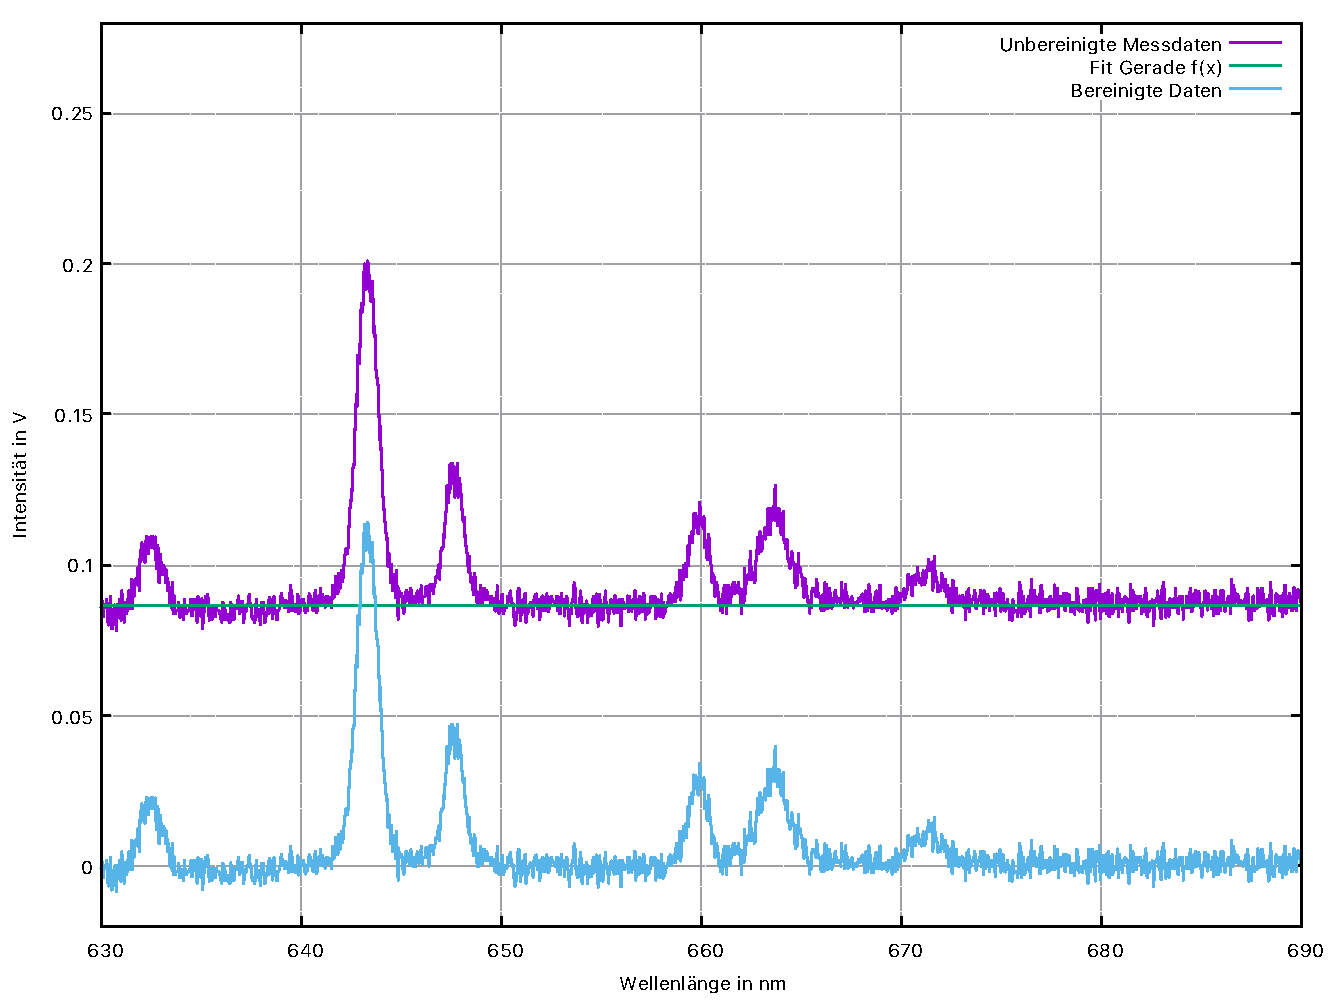
\includegraphics[scale=0.6]{Bilder/Verbesserung_Auswertung/Offset.pdf}
  \caption{Spektrum von $CDCl_3$, im Anti-Stokes Bereich bei 0° Polarisation, zur Veranschaulichung
  der Bereinigung des Offsets  der Messdaten mithilfe einer Fit-Gerade.}
\end{figure}\\
Im Folgenden wird nur noch mit den bereinigten Daten gerechnet.\\
Die veränderten Intensitäten, im Vergleich zu den im Versuch bestimmten, wurden mit der gleichen
Methodik wie während dem Versuch bestimmt.
\newpage
\subsection{Berechnung des Depolarisationsgrad}
Hierzu wird die im Skript angegebene Formel verwendet:\\
\begin{equation}
    \rho = \frac{I_{\perp}}{I_{\parallel}}
\end{equation}
$\rho$ steht hier für den Depolarisationsgrad, dieser berechnet sich aus 
dem Verhältnis der senkrecht bzw. parallel zur einfallenden Strahlung polarisierten Anteile
des Streulichts. \\
Die parallele Intensität ist die Intensität bei der der Polarisator und Analysator 
in die gleiche Richtung zeigen, in unserem Fall ist der Analysator vertikal ausgerichtet
gewesen. Bei uns gilt also: \\
\begin{equation}
    \rho = \frac{I_{\perp}}{I_{\parallel}} = \frac{I_{0^{\circ}}}{I_{90^{\circ}}}
\end{equation}
Zur Berechnung des Depolarisationsgrade werden die Peak-Intensitäten bei 0° und 90° bestimmt. Jedoch ist es 
logisch, das nur die Peaks verwendet werden können, die sowohl bei dem Spektrum mit 0° bzw. 90° erkennbar sind.\\
Als Beispiel soll die folgende Grafik dies veranschaulichen:
\begin{figure}[h]
  \centering
  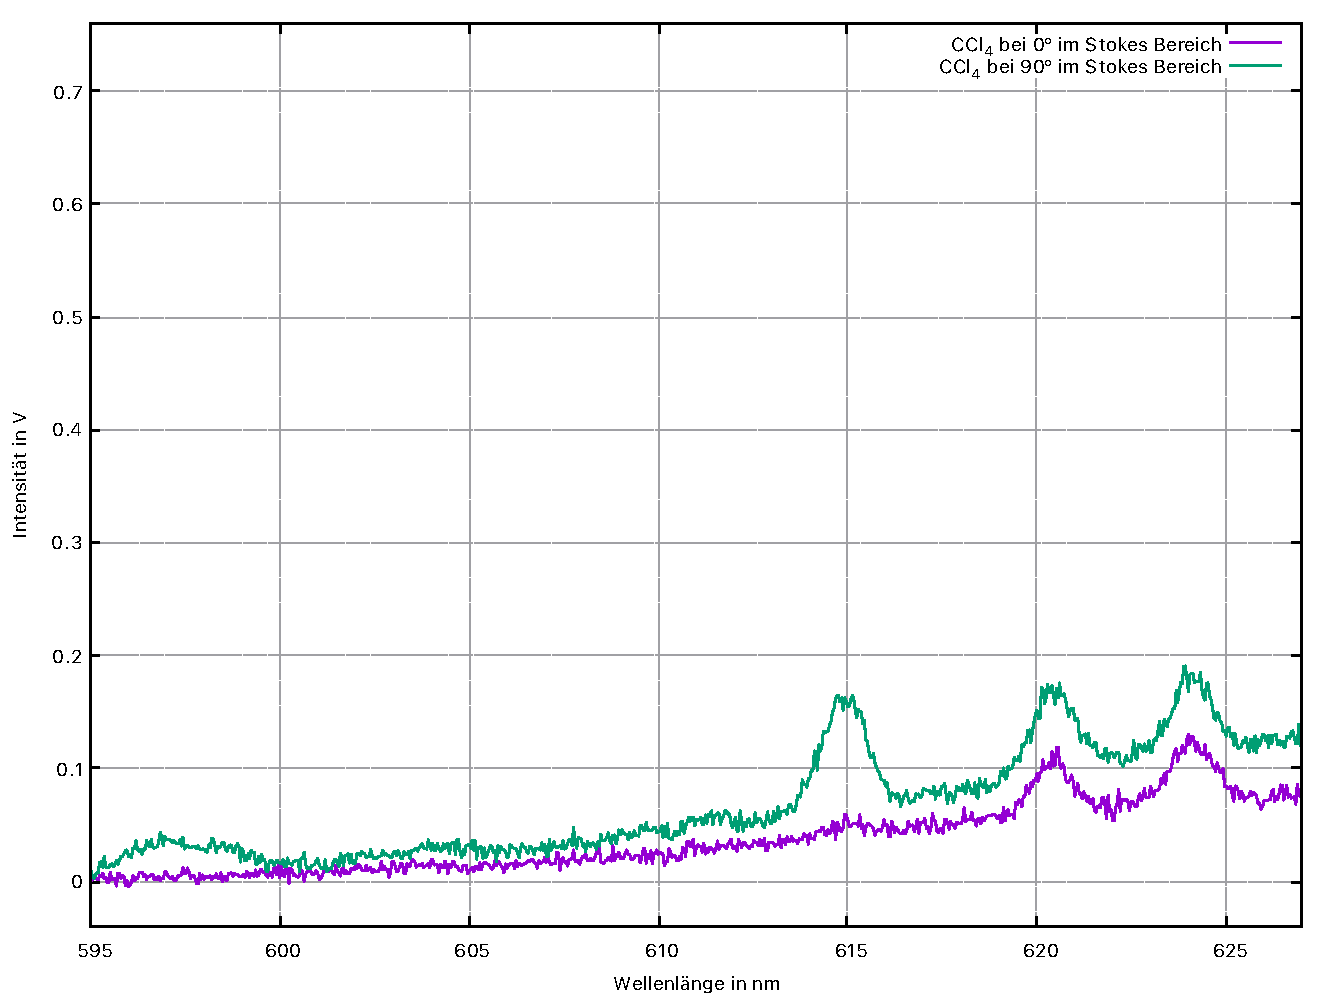
\includegraphics[scale=0.6]{Bilder/Verbesserung_Auswertung/Depol.pdf}
  \caption{Spektrum von $CCl_4$, im Stokes Bereich bei 0° und 90°. Zur Veranschaulichung der Peak-Intensitäten Bestimmung.}
\end{figure}\\
Wie man erkennen kann, liegt ein Peak bei 90° Polarisation bei ungefähr  $\lambda = 595\,nm$. Dieser Peak ist allerdings nicht
bei einer Polarisation von 0° erkennbar. Somit kann dieser auch nicht bei der Depolarisationsgradbestimmung (vgl. Tabelle \ref{tab:ccl4}) berücksichtigt werden.\\
Die restlichen Spektren sind im Anhang zu finden.
\newpage
Der Fehler des Depolarisationsgrad wird mithilfe der Fehlerfortpflanzung berechnet:
\begin{equation}
    s_{\rho} = \sqrt{\left(\frac{I_{\perp}}{I^2_{\parallel}} \cdot s_{I_{\parallel}} \right)^2 + \left(\frac{1}{I_{\parallel}} \cdot s_{I_{\perp}} \right)^2}
\end{equation}
Die Ablesefehler der Intensitäten wurde abgeschätzt: 
$s_{I_{\perp}} = s_{I_{\parallel}} = 0,005\,\text{V}$.\\
Somit erhält man die Folgende Werte:\\
\begin{table}[h]
  \centering
    \begin{tabular}{c||c|c|c|c}
    \makecell{Wellenlänge\\ in nm} & Intensität $I_{0^{\circ}}$ in V & Intensität $I_{90^{\circ}}$ in V & Depolarisation $\rho$ & \makecell{Fehler des \\ Depolarisationsgrad $s_{\rho}$} \\
    \hline
    618,4 & 0,01262 & 0,06726 & 0,1877 & 0,0756 \\
    622,4 & 0,04525 & 0,06828 & 0,6627 & 0,0878 \\
    628,4 & 0,01556 & 0,02638 & 0,5898 & 0,2201 \\
    \end{tabular}%
    \caption{Tabelle über die Wellenlänge der bestimmten Peaks von $CHCl_3$ im Stokesbereich, mit den entsprechenden Intensitäten für 0° und 90° Polarisation sowie dem Depolarisationsgrad und dessen Fehler. }
\end{table}

\begin{table}[h]
  \centering
    \begin{tabular}{c||c|c|c|c}
        \makecell{Wellenlänge\\ in nm} & Intensität $I_{0^{\circ}}$ in V & Intensität $I_{90^{\circ}}$ in V & Depolarisation $\rho$ & \makecell{Fehler des \\ Depolarisationsgrad $s_{\rho}$} \\
        \hline
      643,3 & 0,12102 & 0,16876 & 0,7171 & 0,0365 \\
      647,7 & 0,04695 & 0,24990 & 0,1879 & 0,0204 \\
      660,7 & 0,02184 & 0,22790 & 0,0958 & 0,0220 \\
      664,9 & 0,02812 & 0,03461 & 0,8123 & 0,1861 \\
      685,3 & 0,00879 & 0,01382 & 0,6359 & 0,4287 \\  
    \end{tabular}
    \caption{Tabelle über die Wellenlänge der bestimmten Peaks von $CHCl_3$ im Anti-Stokesbereich, mit den entsprechenden Intensitäten für 0° und 90° Polarisation sowie dem Depolarisationsgrad und dessen Fehler. }
\end{table}

\begin{table}[h]
    \centering
    \begin{tabular}{c||c|c|c|c}
      \makecell{Wellenlänge\\ in nm} & Intensität $I_{0^{\circ}}$ in V & Intensität $I_{90^{\circ}}$ in V & Depolarisation $\rho$ & \makecell{Fehler des \\ Depolarisationsgrad $s_{\rho}$} \\
      \hline
      620,5 & 0,11861 & 0,17082 & 0,6943 & 0,0356 \\
      624,1 & 0,12261 & 0,18396 & 0,6665 & 0,0327 \\  
    \end{tabular}%
    \caption{Tabelle über die Wellenlänge der bestimmten Peaks von $CCl_4$ im Stokesbereich, mit den entsprechenden Intensitäten für 0° und 90° Polarisation sowie dem Depolarisationsgrad und dessen Fehler. }
    \label{tab:ccl4}
\end{table}

\begin{table}[h]
  \centering
    \begin{tabular}{c||c|c|c|c}
      \makecell{Wellenlänge\\ in nm} & Intensität $I_{0^{\circ}}$ in V & Intensität $I_{90^{\circ}}$ in V & Depolarisation $\rho$ & \makecell{Fehler des \\ Depolarisationsgrad $s_{\rho}$} \\
      \hline  
      641,5 & 0,14366 & 0,20090 & 0,7151 & 0,0306 \\
      645,7 & 0,14717 & 0,22574 & 0,6520 & 0,0264 \\
      651,7 & 0,07072 & 0,51630 & 0,1370 & 0,0098 \\
      665,5 & 0,03812 & 0,06580 & 0,5793 & 0,0878 \\
    \end{tabular}%
    \caption{Tabelle über die Wellenlänge der bestimmten Peaks von $CCl_4$ im Anti-Stokesbereich, mit den entsprechenden Intensitäten für 0° und 90° Polarisation sowie dem Depolarisationsgrad und dessen Fehler. }
  \end{table}
\newpage
Die zu erwartenden Depolarisationsgrad-Werte sollten im Bereich $0 < \rho < 0,75$ liegen.\\
Raman-Linien mit $\rho = 0$ sind vollständig polarisiert und Linien mit 
$\rho = \frac{3}{4}$ sind depolarisiert. Unsere Werte des Depolarisationsgrad für die beiden Moleküle 
$CCl_4$ und $CHCl_3$ stimmen somit mit den Erwartungen überein.  \\
Ein kleiner Polarisationsgrad bedeutet, dass die Schwingung symmetrisch ist. Einige Beispiele hierfür
sind beim Molekül $CHCl_3$ die Raman-Linien bei einer Wellenlänge von $647,7\,$nm und $660,7$\,nm 
und beim Molekül $CCl_4$ die Linie bei 
651,7\,nm. \\
Im umgekehrten Fall ist die Schwingung antisymmetrisch. Einige Beispiele sind
beim Molekül $CHCl_3$ die Linien der Wellenlängen 622,4\,nm sowie 643,3\,nm und beim Molekül 
$CCl_4$ die Linie bei einer Wellenlänge von 624,1\,nm.
Diese Werte passen im groben mit den Literaturwerten überein \citep[vgl.][]{zusatzliteratur}.\\
Wie allerdings zu erkennen ist, sind einige der Fehler des Depolarisationsgrades ziemlich hoch, das hängt mit der ungenauen Bestimmung
der Peak-Intensitäten zusammen.

